\section{Experiments and Discussion}
\label{sec:results}

\begin{table}[t]
\centering
\caption{Part~1: \texttt{EncDec} vs.\ \texttt{U-Net} (BCE) on PH2 ($256\times256$) and DRIVE ($512\times512$).}
\label{tab:main_results}
\scriptsize
\begin{tabular}{@{}lllccccc@{}}
\toprule
Dataset & Model & Split & Dice & IoU & Acc & Sens & Spec \\
\midrule
PH2 & EncDec & Train & 0.9439 & 0.8937 & 0.9627 & 0.9682 & 0.9601 \\
PH2 & EncDec & Val   & 0.9302 & 0.8696 & 0.9497 & 0.9495 & 0.9498 \\
PH2 & EncDec & Test  & 0.8750 & 0.7777 & 0.9269 & 0.8919 & 0.9410 \\
\midrule
PH2 & U-Net  & Train & 0.9373 & 0.8819 & 0.9593 & 0.9395 & 0.9688 \\
PH2 & U-Net  & Val   & 0.9371 & 0.8816 & 0.9559 & 0.9287 & 0.9708 \\
PH2 & U-Net  & Test  & \textbf{0.8796} & \textbf{0.7851} & \textbf{0.9316} & 0.8715 & \textbf{0.9558} \\
\midrule
DRIVE & EncDec & Train & 0.4065 & 0.2551 & 0.9198 & 0.3199 & 0.9761 \\
DRIVE & EncDec & Val   & 0.4407 & 0.2826 & 0.9192 & 0.3808 & 0.9683 \\
DRIVE & EncDec & Test  & 0.4222 & 0.2676 & 0.9185 & 0.3266 & 0.9779 \\
\midrule
DRIVE & U-Net  & Train & 0.8198 & 0.6946 & 0.9698 & 0.8002 & 0.9857 \\
DRIVE & U-Net  & Val   & 0.7997 & 0.6662 & 0.9669 & 0.7910 & 0.9829 \\
DRIVE & U-Net  & Test  & \textbf{0.7993} & \textbf{0.6658} & \textbf{0.9653} & \textbf{0.7577} & \textbf{0.9862} \\
\bottomrule
\end{tabular}
\end{table}

\subsection{Architecture & Loss Ablations (Part 1)}
As shown in Table~\ref{tab:main_results}, \texttt{EncDec} performs well on PH2 ($\text{Test Dice}=0.8750$) due to large lesions, while \texttt{U-Net} reaches $0.8796$. On DRIVE, \texttt{EncDec} fails to capture thin vessels ($\text{Test Dice}=0.4222$, $\text{Sens}=0.3266$), whereas \texttt{U-Net} skip connections nearly double Test Dice to $0.7993$ ($\text{Sens}=0.7577$).

In Table~\ref{tab:loss_ablation}, Focal Loss ($\gamma=2$) achieves the best PH2 Test Dice ($0.8823$) by emphasizing hard boundaries. On DRIVE, Weighted BCE ($w=8$) boosts vessel Sensitivity ($0.7577 \to 0.8276$) but lowers Specificity ($0.9862 \to 0.9721$) and Dice ($0.7993 \to 0.7860$) due to thicker boundary false positives.

\begin{table}[t]
\centering
\caption{Part~1: Loss ablation on \texttt{U-Net} (Test split).}
\label{tab:loss_ablation}
\scriptsize
\begin{tabular}{@{}llccccc@{}}
\toprule
Dataset & Loss & Dice & IoU & Acc & Sens & Spec \\
\midrule
PH2 & BCE                 & 0.8796 & 0.7851 & 0.9316 & 0.8715 & \textbf{0.9558} \\
PH2 & Focal ($\gamma=2$)  & \textbf{0.8823} & \textbf{0.7894} & \textbf{0.9324} & 0.8844 & 0.9516 \\
PH2 & Weighted BCE ($w=2$)& 0.8789 & 0.7840 & 0.9288 & \textbf{0.9011} & 0.9399 \\
\midrule
DRIVE & BCE                 & \textbf{0.7993} & \textbf{0.6658} & \textbf{0.9653} & 0.7577 & \textbf{0.9862} \\
DRIVE & Focal ($\gamma=2$)  & 0.7963 & 0.6616 & 0.9645 & 0.7604 & 0.9850 \\
DRIVE & Weighted BCE ($w=8$)& 0.7860 & 0.6475 & 0.9589 & \textbf{0.8276} & 0.9721 \\
\bottomrule
\end{tabular}
\end{table}

\subsection{Weak Point Supervision on PH2 (Part 2)}
Table~\ref{tab:weak_results} shows that \texttt{U-Net} trained with only $1+1$ clicks already reaches $0.7202$ Test Dice, rising steadily with $5+5$ ($0.8345$) and $10+10$ ($0.8592$). At $25+25$ clicks ($50$ pixels/image, $<0.08\%$ of $256^2$), weak supervision reaches $0.8808$ Test Dice, matching full supervision ($0.8796$) before saturating at $50+50$ ($0.8769$). Comparing sampling strategies at $10+10$ clicks, \texttt{Interior} slightly improves Val Dice ($0.9068$ vs.\ $0.9031$) and Test Specificity ($0.9665$ vs.\ $0.9567$) but lowers Sensitivity ($0.8058$ vs.\ $0.8342$) because avoiding boundary clicks removes border supervision, causing slight under-segmentation.

\begin{table}[t]
\centering
\caption{Part~2: Weak point-click supervision on PH2 (\texttt{U-Net}, Test split) vs.\ full supervision ($65{,}536$ px/img).}
\label{tab:weak_results}
\scriptsize
\begin{tabular}{@{}llccccc@{}}
\toprule
Clicks (pos+neg) & Strategy & Dice & IoU & Acc & Sens & Spec \\
\midrule
1 + 1   & Uniform  & 0.7202 & 0.5627 & 0.8407 & 0.7148 & 0.8914 \\
5 + 5   & Uniform  & 0.8345 & 0.7160 & 0.9040 & 0.8444 & 0.9279 \\
10 + 10 & Uniform  & 0.8592 & 0.7531 & 0.9216 & 0.8342 & 0.9567 \\
10 + 10 & Interior & 0.8531 & 0.7438 & 0.9204 & 0.8058 & \textbf{0.9665} \\
25 + 25 & Uniform  & \textbf{0.8808} & \textbf{0.7870} & 0.9301 & \textbf{0.9003} & 0.9422 \\
50 + 50 & Uniform  & 0.8769 & 0.7807 & 0.9310 & 0.8568 & 0.9608 \\
\midrule
Full Mask & Full   & 0.8796 & 0.7851 & \textbf{0.9316} & 0.8715 & 0.9558 \\
\bottomrule
\end{tabular}
\end{table}

\begin{figure*}[t]
\centering
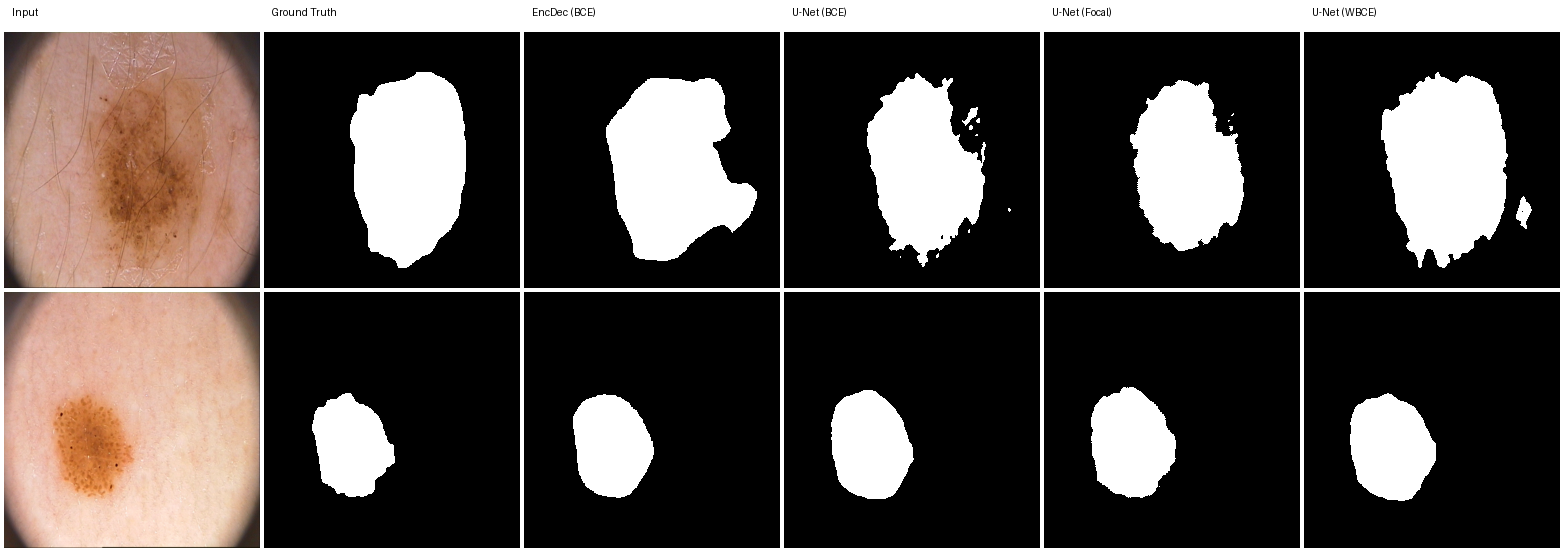
\includegraphics[width=0.95\textwidth]{fig/qualitative_ph2.png}\\[3pt]
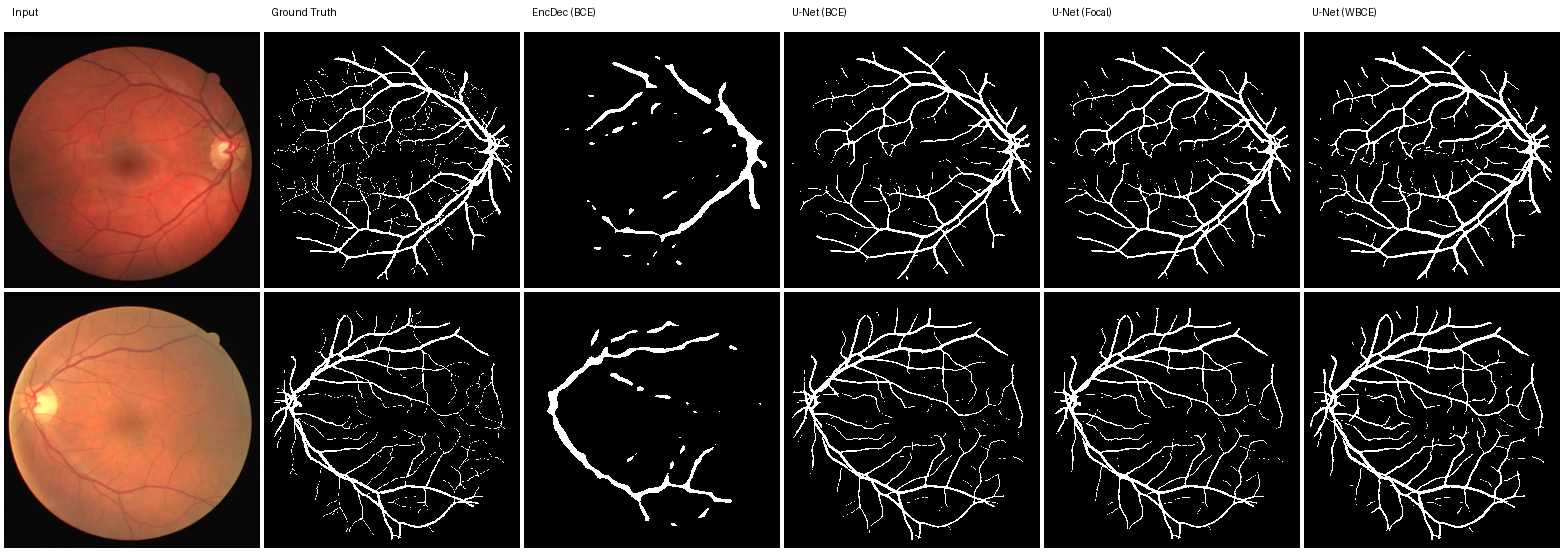
\includegraphics[width=0.95\textwidth]{fig/qualitative_drive.png}
\caption{Qualitative test-set predictions on PH2 (top two rows) and DRIVE (bottom two rows). \texttt{U-Net} recovers fine retinal vessel structures missed by \texttt{EncDec}, while Weighted BCE increases vessel sensitivity at the expense of thicker boundary predictions.}
\label{fig:qualitative}
\end{figure*}
